\chapter{Studi Literatur}

Pada bab ini, akan diisi oleh studi literatur, hal-hal yang berkaitan dengan topik persoalan tugas akhir akan dipaparkan dalam bab ini guna untuk memberikan informasi mengenai dasar teori dan studi yang dipakai. Bab ini diharapkan membantu pembaca untuk mengerti dalam membaca penelitian tugas akhir ini.

\section{\textit{Information Retrieval}}
\textit{Information Retrieval} (IR) adalah penemuan bahan seperti dokumen yang bersifat terstruktur yang memenuhi kebutuhan informasi dari dalam koleksi besar yang tersimpan di dalam komputer \parencite{introtoinforetri}. IR saat ini sangat sering dilakukan contohnya dalam pencarian informasi berkaitan dengan representasi, penyimpanan, pengaturan, dokumen, halaman web, katalog online, catatan, dan objek multimedia. 

\section{Apache Lucene}
Apache Lucene adalah \textit{library search engine} yang berperforma tinggi dan berfitur lengkap yang seluruhnya ditulis dalam Java. Apache Lucene cocok untuk aplikasi yang memerlukan pencarian terstruktur, pencarian teks lengkap, pencarian pada graf dengan banyak node maupun vektor derajat tinggi, koreksi ejaan, atau saran kueri \parencite{apachelucene}.

\section{Elastic Search}
Elasticsearch adalah aplikasi mesin pencarian RESTful. Elastic Search menyimpan data secara terpusat untuk pencarian secepat kilat dan paling relevan \parencite{elasticsearchorigin}. Elastic Search diciptakan sebagai pembungkus dan inovasi dari Apache Lucene yang sekedar hanya \textit{library} karena aplikasi yang beredar saat ini tidak hanya dibuat di atas Java dan membutuhkan fleksibilitas yang tinggi, sedangkan, Apache Lucene terkenal sangat sulit untuk orang awam yang tidak memahami istilah-istilah dan \textit{information retrieval}. Elastic Search sendiri dibuat menggunakan Java namun menggunakan \textit{Application Programming Interface} RESTful melalui protokol HTTP sehingga aplikasi dengan bahasa apapun dapat dengan mudah menggunakan aplikasi ini. Tidak hanya itu, API dari Elastic Search ini juga sudah sangat dipermudah sehingga pemakai tidak perlu mengetahui istilah-istilah dalam Apache Lucene. Sehingga, Elastic Search ini sangat dekat dengan proses umum pada data seperti menyimpan, membaharui, menghapus, pengindeksan, pencarian, dan sebagainya.

\section{Java \textit{Virtual Machine}}
\textit{Java Virtual Machine} atau JVM adalah program yang dapat membaca program java yang telah dikompilasi atau biasa dikenal sebagai \textit{java bytecode} dan menginterpretasikannya menjadi bahasa mesin yang dapat dieksekusi oleh komputer \parencite{java12}. Struktur JVM terdiri dari \textit{runtime data structure} di memori dan dua subsistem yang berhubungan langsung dengan \textit{runtime data structure} yaitu \textit{class loader} dan \textit{execution engine}. Semua program yang dibuat dengan Java akan dikompilasi ke \textit{java bytecode} yang nantinya akan diinterpretasikan oleh JVM untuk dieksekusi komputer. 

\section{\textit{Indexing and Caching}}
Kita dapat mencari halaman yang berisikan suatu topik atau kata kunci pada sebuah buku teks dengan melihat indeks sebuah buku. Indeks disusun secara terurut dan mengurangi usaha untuk mencari suatu hal yang diinginkan oleh penggunanya. Secara umum, indeks pada sebuah file di sebuah basis data berlaku sama pada indeks di buku teks, \parencite{database}.

Konsep \textit{caching} sendiri adalah menyimpan data yang sering diakses pada level cache atau memori yang lebih dekat dengan CPU agar dapat diakses dengan cepat saat ingin melakukan pencarian, lihat gambar \ref{fig:level-cache}. \textit{Cache} sendiri biasanya memiliki ruang yang terbatas sehingga biasanya membuang data yang sudah tidak diakses sehingga jika dibutuhkan harus dicari ke \textit{storage}. Konsep ini ditiru oleh basis data dan aplikasi \textit{information retrieval} untuk mempercepat proses pencarian dengan memanfaatkan \textit{indexing} untuk mencari (lihat gambar \ref{fig:cache-app}) dan \textit{caching} untuk mengembalikan data yang sering diakses dengan memanfaatkan memori.

\begin{figure}[h]
    \centering
    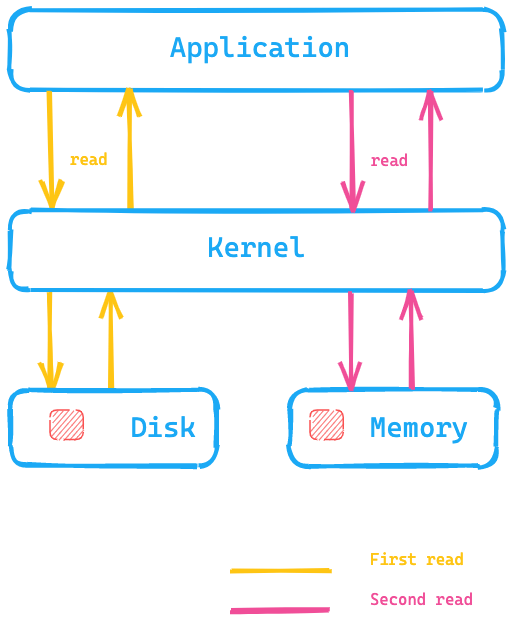
\includegraphics[width=0.5\textwidth]{chapter-2/cache-app.png}
    \caption{Prinsip Cache pada Aplikasi}
    \label{fig:cache-app}
\end{figure}

\begin{figure}[h]
    \centering
    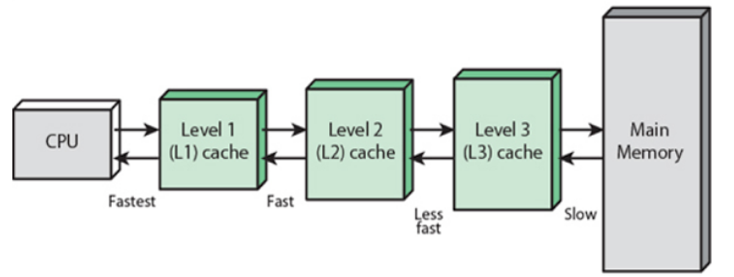
\includegraphics[width=0.5\textwidth]{chapter-2/cache-memory.jpeg}
    \caption{Level-level pada Cache}
    \label{fig:cache-level}
\end{figure}

\section{Kubernetes}

\subsection{Pod}
Pod adalah unit komputasi terkecil yang dapat dibuat dan dikelola dalam Kubernetes. Pod berisi lebih dari satu kontainer dan memiliki jaringan serta penyimpanan yang dipakai bersama serta spesifikasi untuk menjalankan kontainer didalamnya, \parencite{pod}.

\subsection{\textit{Autoscaler}}
\textit{Autoscaler} adalah komponen yang mengatur alokasi sumber daya komputasi secara dinamis yang disesuaikan dengan beban layanan pada saat tertentu. Saat ini di Kubernetes, terdapat dua pendekatan \textit{Autoscaling} 

\subsubsection{\textit{Horizontal Autoscaler}}
\textit{Horizontal Autoscaler} fokus untuk melakukan penskalaan dengan bantuan replikasi. \textit{Kubernetes Horizontal Pod Autoscaler} secara otomatis akan menlakukan penskalaan jumlah pod yang di-\textit{deploy} sehingga dapat menyesuaikan dengan kebutuhan dengan cara menambah atau mengurangi replikasi yang ada, \parencite{hpa}. 

\subsubsection{\textit{Vertical Autoscaler}}
Berbeda dengan cara horizontal, \textit{Vertical Autoscaler} lebih fokus untuk mengubah ukuran alokasi utilisasi pada pod yang ada. \textit{Kubernetes Vertical Pod Autoscaler} berguna untuk mengotomasi reservasi CPU dan memori yang sesuai. Penyesuaian ini dapat meningkatkan kluster kubernetes spesifiknya pada utilitasi sumber daya karena dapat mengurangi alokasi CPU dan memori pada sebuah \textit{node} agar bisa dipakai oleh pod lain, \parencite{vpa2}.

\subsection{\textit{Kubernetes Client Library}}
\textit{Kubernetes Client Library} berguna untuk melakukan operasi-operasi pengelolaan terutama autentikasi sebuah kluster kubernetes melalui API, \parencite{clientlibrary}. Saat ini, Kubernetes sudah memiliki \textit{library} resmi pada bahasa pemrograman, diantaranya.

\begin{enumerate}
    \item C (https://github.com/kubernetes-client/c),
    \item Dotnet (https://github.com/kubernetes-client/csharp),
    \item Golang (https://github.com/kubernetes/client-go/),
    \item Java (https://github.com/kubernetes-client/java),
    \item Python (https://github.com/kubernetes-client/python/),
    \item Haskell, Ruby, Perl, dan Javascript.
\end{enumerate}

\section{Pembelajaran Mesin}
Pembelajaran Mesin adalah sebuah bidang pembelajaran yang mempelajari pemahaman dan membangun metode untuk "belajar" dengan memanfaatkan data untuk meningkatkan banyak aspek terutama efisiensi dan kualitas terhadap suatu rangkaian tugas. Algoritma pembelajaran mesin membangun model berdasarkan data sampel yang biasa disebut \textit{training data} untuk menghasilkan model yang dapat memprediksi atau membuat keputusan tanpa diprogram secara eksplisit, \parencite{ml}.

\subsection{\textit{Reinforcement Learning}}
\textit{Reinforcement learning} atau RL adalah bidang pembelajaran mesin yang mengotomasi sebuah agen untuk mengambil tindakan dan memaksimalkan \textit{reward} dari aksi yang dilakukan, \parencite{reinforcementlearning}. RL adalah salah satu paradigma dari tiga pembelajaran mesin dasar seperti \textit{Supervised Learning} dan \textit{Unsupervised Learning}. Singkatnya, RL membuat agen dapat mengoreksi pengetahuannya secara terus menerus agar dapat memaksimalkan fungsinya. Berbeda dengan \textit{Supervised Learning}, RL tidak memerlukan label dan tidak memerlukan secara eksplisit dikoreksi. Fokus dalam membangun RL, adalah mencari keseimbangan eksplorasi terhadap lingkungan baru dan eksploitasi terhadap pengetahuan yang dimiliki.